\section {库存管理}

-

    \begin{center}
        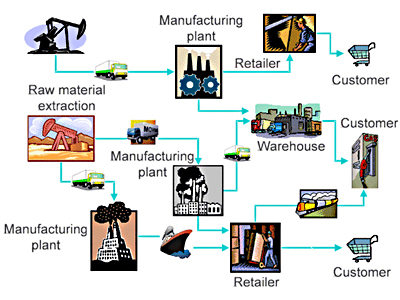
\includegraphics[scale=1.5] {factory.jpg}
    \end{center}

    库存是企业组织中存储的各种物品与资源的总和,是企业在生产和物流渠道中各仓库堆积的原材料、供给品、零部件、半成品和成品等。库存是企业进行正常生产经营活动所必须具备的条件,在企业生产经营过程中,库存能够实现企业的规模经济,满足供求平衡,预防需求和订货周期的不确定性。

    库存管理的宗旨和目标是在保证供应的前提下尽可能的降低成本。库存管理的核心问题是库存控制。库存控制就是确定合理的订货时间和数量,用最少的费用去满足生产和经营的需要。并借以获得最大的经济效益,随着企业走向市场。企业为充分发挥资金的效用,取得较好的经济效益,对库存控制越来越重视。

\subsubsection { 库存对企业的影响}

    如今,企业对库存管理越来越重视,无论它是制造商、分销商、批发商、零售商,或是其他类型的行业企业。因为库存资产在企业总资产额中所占比率相当可观,降低库存是实质性地减少流动资金需求的最快方式之一。库存周转把资产转变为利润,库存周转越快,收益率越好。诸如资产回报率以及其它一些资金使用效率方面的评价越来越普遍地影响着组织。在公司中,库存起着如下五个作用:

    \begin{enumerate}
        \item  使公司有可能达到规模经济;
        \item  平衡供求;
        \item  使制造专业化成为可能;
        \item  保护公司少受需求和订货周期的影响;
        \item  在分配渠道间起缓冲器作用。
    \end{enumerate}

\subsubsection { 库存对物流的影响}

    从某种意义上讲,仓储管理在物流管理中占据着核心的地位。这是因为库存总是出现在物流各环节的接合部,例如采购与生产之间,生产的初加工与精加工之间,生产与销售之间,批发与零售之间,不同运输方式转换之间等等。仓储是物流各环节之间存在不均衡性的表现,库存也正是解决这种不均衡性的手段。仓储环节集中了上下游流程整合的所有矛盾,库存管理就是在实现物流流程的整合。如果借用运筹学的语言来描述仓储管理在物流中的地位,可以说就是在运输条件为约束力的情况下,寻求最优库存(包括布局)方案作为控制手段,使得物流达到总成本最低的目标。在许多具体的案例中,物流的整合、优化实际上归结为仓储的方案设计与运行控制。

\subsection {库存控制}

    库存信息对财务的资产负债表和损益表有直接的关系。 库存是可以交换和销售的流动资产,一般约占企业资产的 20\%~60\%。在损益表中以销售产品成本的形式出现,它是说明企业收益的重要因素。库存反映了企业财务状况的好坏。因此,库存管理非常重要,不能仅仅看成是一个记好库存台账的问题。

    库存管理因计划与控制的层次(独立需求件、相关需求件)、物料对象(产品、在制品、半成品、原材料、MRO)、物料的 ABC 分类、 供需链上的地位(供应、制造、分销)、物料供应周期的长短而异。在供需链上每一个经济实体之间,都有可能出现库存和运输。

    在 APICS 词汇中 “库存 (inventory)” 一词的定义是: “以支持生产、维护、操作和客户服务为目的而存储的各种物料;包括原材料和在制品、维修件和生产消耗品、成品和备件等”。

    因此,库存管理主要是: “与库存物料的计划与控制有关的业务”,目的是支持生产运作。注意,不要把它同仓库管理系统〈WMS〉混淆起来。仓库管理系统主要针对仓库或库房的布置、物料运输和搬运、存储自动化等的管理。两者的概念是不同的。

    库存是计划的结果,又是支持计划实现的先决条件。因此,库存管理的首要任务是根据产品计划的要求来控制库存。传统管理习惯把库存管理理解为仅仅是物料的 “入库、存储、出库”,也就是库存事务的一部分工作,这是不全面的。库存管理如果不同计划管理结合起来,就不能说明库存物料的品种,数量和存储时间是否合理,即不能说明库存物料在数量上是存多了还是存少了,在时间上是存早了还是存晚了。库存量应当是计划的结果,库存脱离了计划,就谈不上控制。库存管理除了保证库存信息准确,满足客户和市场需求计划外,一项重要任务是控制库存量,加速库存周转,降低成本。换句话说,评价库存管理的标准主要是

    \begin{itemize}
        \item 客户服务水准,既保证生产和销售的需求又控制资金占用;
        \item 库存占用的资金额,控制在企业预算之内;
        \item 库存资金周转次数,超过、保持或接近行业领先水平。
    \end{itemize}

    库存周转次数计算公式\eqref{eq:inventoryCycle}如下:

    \begin{equation} \label{eq:inventoryCycle}
        库存资金周转次数(次)=
            \cfrac{ \displaystyle 产品年销售成本(元)}{ \displaystyle 库存年平均占用资金额(元)}
    \end{equation}

    这里考核的只是库存资金占用,而不是企业全部流动资金。换句话说,只是流动资金中的盘存资产部分,即储备资金、生产资金和成品资金,不包括结算(如应收账款)和货币资金。这样处理,同成本计算采用制造成本法是一致的。它反映丁企业的库存管理水平。在考核企业业绩时,库存资金周转次数是一项重要的指标,说明为了实现某个销售金额需要用于库存的流动资金的金额数。通过实施 ERP,既要增加销售收入,又要提高库存资金周转次数。通俗地说,就是一个钱能顶几个钱用。库存占用资金同销售收入两者之间并不存在必然的线性关系,管理的目标是:既要增加销售收入又要降低库存资金占用。

    库存控制同计划层次对应,也有宏观和微观两个层次。宏观层主要控制会计年度内的库存水准,作为财务预算的依据。控制库存水准的主要参考值是同行业类似企业在类似客户服务水准下的库存周转次数。按照高标准定位的精视应高于同行业的平均库存周转次数。

    微观层主要针对库存事务、盘点及储运等,也就是软件中库存管理的主要功能。日本的JIT哲理,把库存量比作江湖的水量,把水下的礁石比作由于管理不善造成的各种问题,如预测不准、供应不及时、计划不周、能力不足、质量不高、不重视培训、设备保养差等等。库存量大了相当于水位高了,淹没了水下的礁石,看上去有利于通航,但是水下被掩盖了的问题(瞧石)却馗不能暴露出来,也永远手寻不到彻底解决。因此,库存量过大被喻之为 “众弊之源”。就是说,库存量掩盖的管理问题是永远不会自动消除的。如图 \ref{fig:inventoryShip}所示。

    \begin{figure}[h]
        \centering
        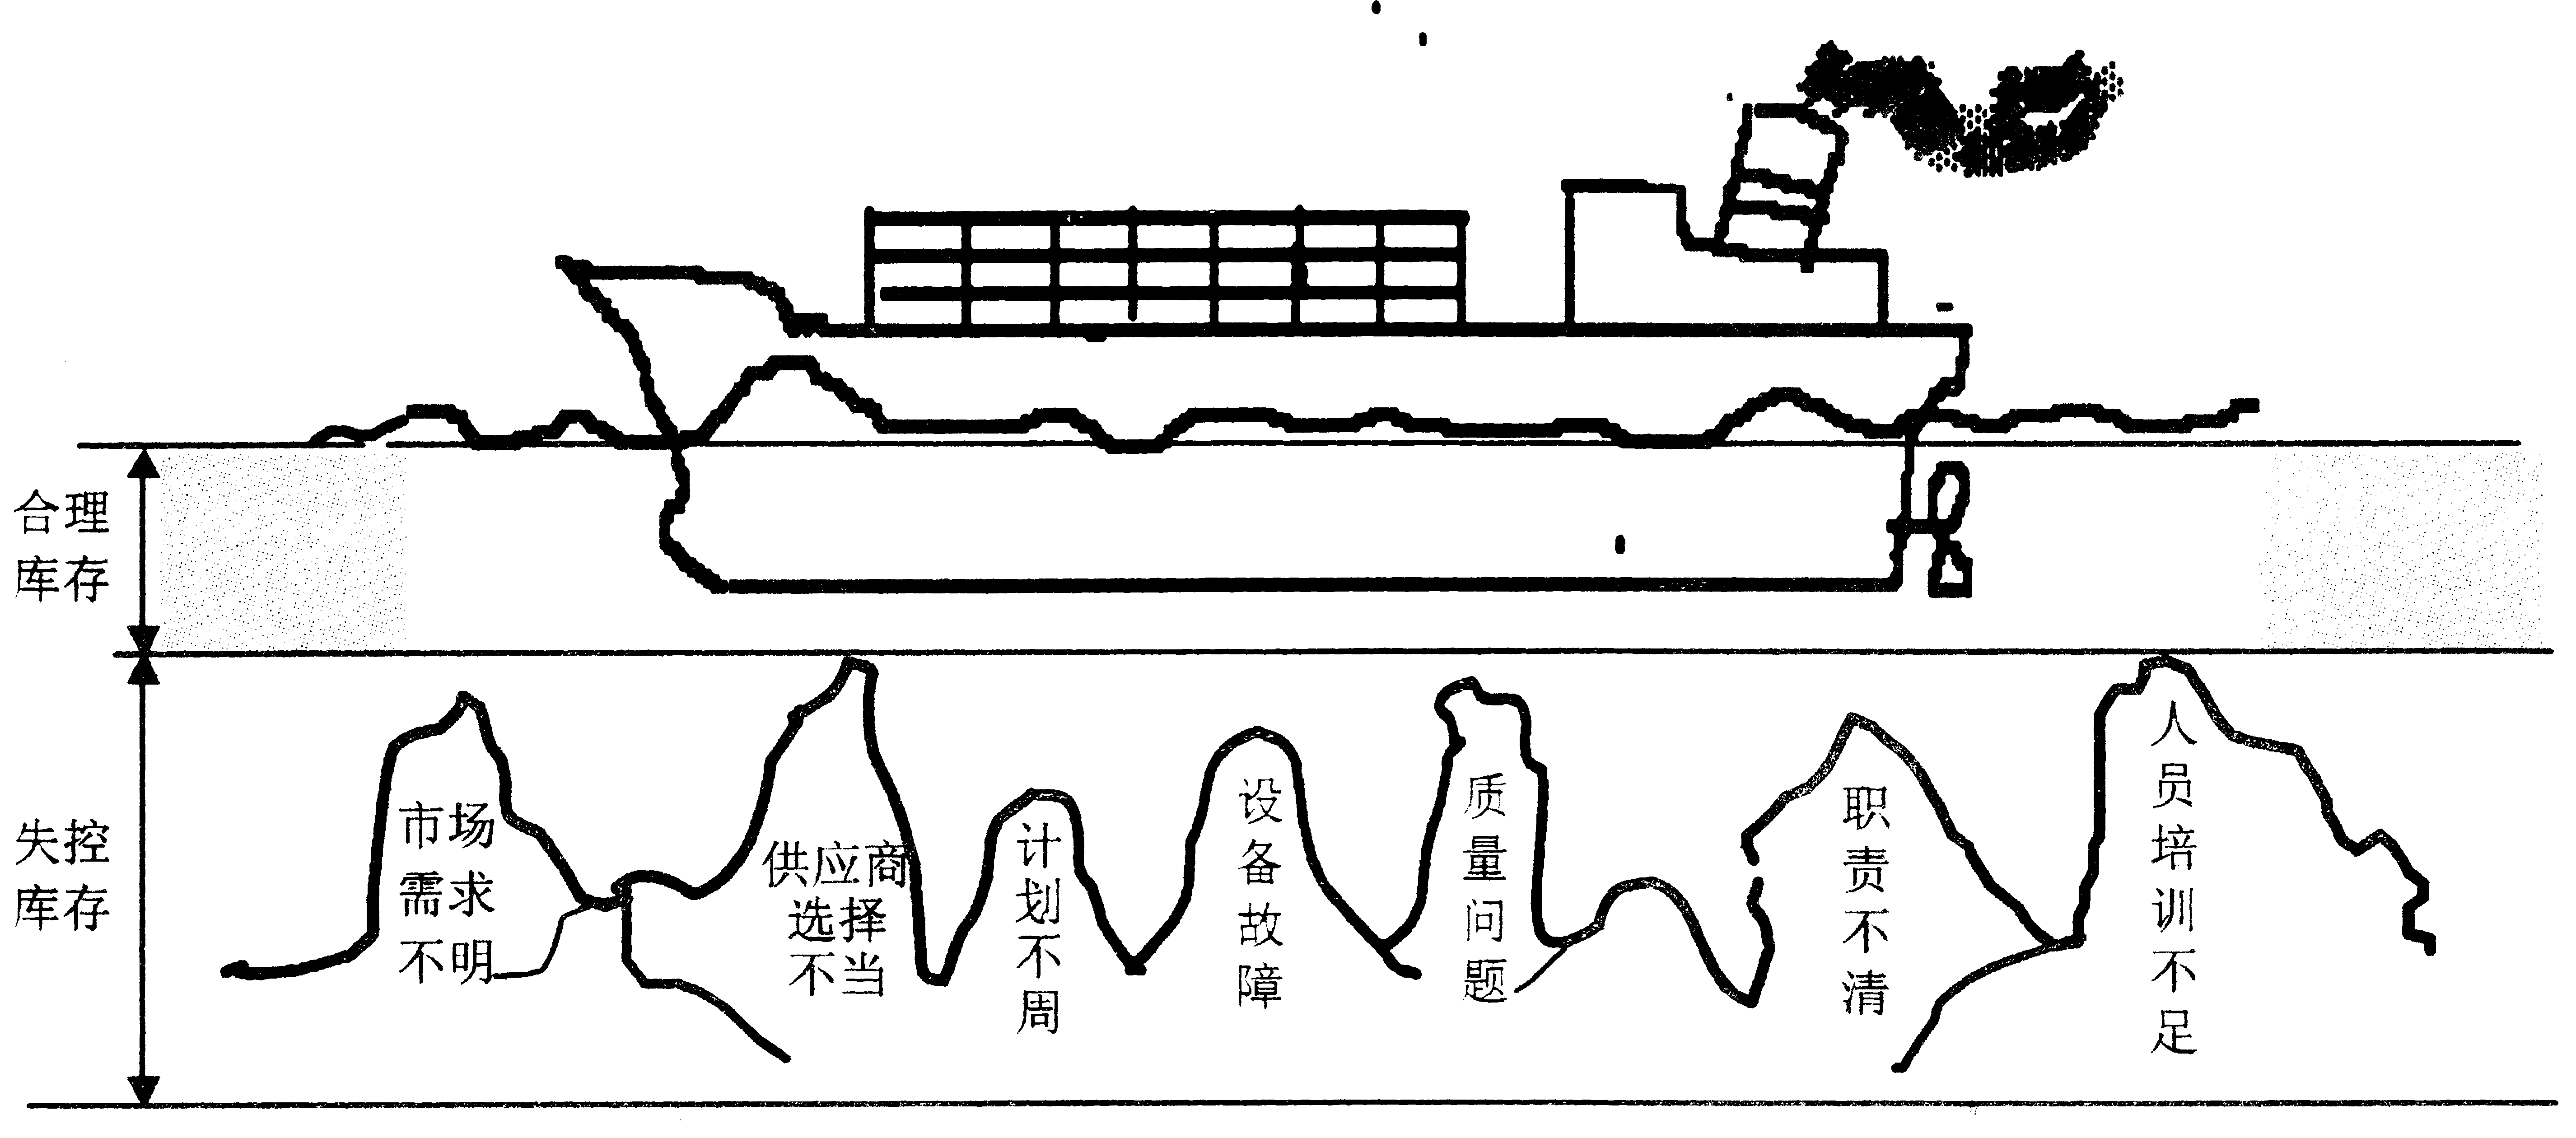
\includegraphics[scale=0.75]{inventoryShip.png}
        \caption{过量库存掩盖管理不善的问题} \label{fig:inventoryShip}
    \end{figure}

    人总是有一些惰性,总是希望工作轻松一点。因此,只有当库存资金占用影响了企业的竞争力或利润时,才会下决心去降低库存。这个要求通常是企业老总提出来的,北京一个汽车厂,平时生产线上储存了 2\~3 天的用量,习以为常,后来老总提出要求降到 10 件,促使员工精心操作,实现了新的目标。真是: “老总不发话,库存降不下”。

    从图 \ref{fig:inventoryShip} 里也可以看出,任何船只都会有一定的吃水量,没有水是不能行船的。这里提出 “合理库存”,而不是 “零库存”。零库存是一种控制库存的哲埋,为的是减少一切无效作业与浪费,要有效地使用各个系统和各种技术。例如: 预测要准,加工周期要短,质量要保证,供应商要可靠等。总之,是追求消除不必要的多余库存,而不是追求 “没有” 库存。一个企业自己可以做到 “零” 库存,但是从供需链管理的角度来看,只是库存转移,或 “嫁祸于人”,把原材料存在供应商的仓库,把产成品存在经销商的仓库。因此,要用整体拥有成本(TCO)全面而系统地权衡。

    控制库存量是物料管理的重要内容,在确定库存量时要注意库存目的和库存费用。

\subsection {库存的目的}

    如果库存没有目的也就没有储存的必要,这督是控制库存时第一个要考虑的问题。库存的目的主要是为了保证生产和销售正常进行,它有 5种常见的基本类型。

    \begin{enumerate.zh}
        \item 安全库存(safety Stock 或 fluctuation inventory)。有时也称最小库存余量(minimum ba1ance)或最低库存。

        企业内外的需求和供给都可能出现偏离计划或预测的情况,会遇到许多不确定因素。为了不中断生产,在计划需求量之外经常保持一定的库存量作为保险储备。安全库存是物料主文件中一项用户设定的参数,当实际库存量低于安全库存量时,系统会自动生成定单建议用户补足安全库存。

        \item 季节性储备(seasona1 stock)或预期储备(anticipation inventory)。

         受季节供应约束的采购件(如农产品)、受季节市场需求约束的产品(如服装、空调机、节日礼品)、或为工厂休假日及因设备计划检修需要事先储备的物料,统称季节性储备或预期储备。 这类库存一股是可以预计的,用销售与运作计划(S\&OP)来规划。

        \item 批量库存(1ot size inventory 或 working stock)。

        受供应、加工、运输、包装或享受折扣优惠等因素的影响。必须按一定的批量生产或采购。由此形成可能超出实际需要的库存称为批量库存。当批量规则是采用固定批量法时,这类库存尤为突出。

        \item 在途库存(transportation inventory 或 pipeline stock)。

        对厂内来讲,在途库存是工序之间因传送、等待、缓冲而形成的在制品库存。对厂外来讲,在途库存是为了保持连续向用户供货或连续满足本厂需求,在运输途中保有一定数量的物料,在分销资源计
    划和流程工业中的管道输送中常出现在途库存。此外,财务与实物对账时,例如,己付款但货物尚未到厂入库,也要用到在途库存来对应“在途材来斗” 账户。

        \item 囤积库存(hedge inventory)。

        针对生产常用物料涨价趋势,储备一定数量,以控制今后成本。由于这样做要积压库存资金,必须分析涨价因素同多付利息之间的关系。如果囤积库存不是生产用的物料,应归入 “不可动用量” 中,不参与需求计算。系统可以按用户规定,把超过设定的 “最长允许存储天数(或货架天数)”,在一个期间内未发生任何事务处理的,或超过规定的 “最大存储量” 的物料显示出来提醒管理人员分析原因并采取措施。

    \end{enumerate.zh}

\subsection {库存的费用}

    控制库存量的第二个要注意的问题是库存费用,确定库存费用要考虑4个因素。

    \begin{enumerate.zh}
        \item 物料价值。

        物料的单位标准成本或计划价格,在物料主文件中记录。

        \item 定货费(acquisition cost或ordering cost)。

        如前所述,“定货” 包括采购和加工两个方面,是指为了获取物料需要支付的费用。如准备定单、洽谈、运输、搬运、验收、办公和管理等费用。定货费同定货批量和次数有关,批量小,定货次数多,定货费就高。定货费或定货成本通常在物料主文件中记录。

        \item 保管费(carrying cost)。

        保管费是指为了保存物料所支付的费用。如利息、折旧、损耗、财产税、保险等。现代管理把占用资金的机会成本(即这笔资金如果没有作为资金占用而是投资在其他方面所能获得的利益),也计入保管费用,机会成本占保管费用的比例往往在40\%以上,照这样计算,保管费可占到库存价值的 20\%\~35\%。保管费通常用占库存价值的百分比来估算,需要在软件的系统参数中设置。以上 3 项数据在经济批量计算中还会用到,各软件会有具体要求。

        \item 短缺损失(cost of stockout)。

        由于物料出现短缺造成停工待料的损失、紧急定货的额外开支。包括加班加点和紧急采购迟未按期交货造成的客户索赔,撤消定货甚至丧失市场等经济损。

    \end{enumerate.zh}

    以上几项费用相互影响,例如,库存量大可能短缺损失加,但保管费高;要降低保管费就要降低批量,但批量小定货次数增加,定货费用增加。控制库存就是要权衡这些费用,使总费用最低,以实现降低成本的目的。

    通常在控制库存时,由企业领导从宏观上提出一个库存水准的要求,在一种紧迫和危机感的压力下,解决各种管理不善的问题,使库存降到看来似乎已不能再降的程度。经过一个时期,运行已经正常,再提出更高的控制库存水准的要求,进一步挖掘潜力,再次降低库存,从而不断降低成本,满足市场竞争的需要。要做到这点 必须要企业领导提出目标,并监督执行。

\subsection {库存事务}

    除了控制库存外,库存管理的日常工作是库存事务处理,库存事务有 4 种类型:

        \begin{enumerate.zh}
            \item 物料存放位置的变化,即物料的移动。例如,从供应商(采购单)到待验区,从待验区到仓库或退货给供应商,从仓库到车间,从车间到检验区或废品库,从发货区到客户(销售合同)等等。

            \item 物料数量的变化。位置的变化会伴随数量的变化。但是,也有存放位置不变,数量却发生变化的情况。例如,盘点后数量的调整等。

            \item 物料价值的变化。在存放位置和数量都未变化的情况下,物料的价值由于质量,过时废弃等原因在金额(标准成本)上的调整。

            \item 物料状态的变化。在下达定单但是尚未付款或到货的情况,在 ERP 系统会把物料处于一种 “定单状态”,而物料到货入库时则处于一种 “实物状态”。
        \end{enumerate.zh}

    以上 4 类处理便于把事务处理同账务处理对应起来,实现物流信息同资金流信息的集成。

    企业应当列出日常经营生产活动中,都有哪些库存事务,并分析这些事务同什么物理位置发生关系,涉及哪些会计科目,借贷关系如何,又涉及哪些定单。在软件中对每一种库存事务都要有代码并明确定义。

    在分析库存事务的同时,要分析相关的业务流程是否合理。就是说,定义库存事务的过程也是发现业务流程存在问题的过程。
